This section contains the main problem for this project and the form of solution required.

\subsection{The problem}
The analysis was based on the initial problem: \textit{How can the current \citybike system be improved, in order to make it more usable?}.
From the analysis, it was found that the current \citybike has several problems, limiting the overall usability (as described in \cref{aalborg_bycyklen:challenges}).

The main problems identified were:
\begin{enumerate}
\item Bikes left outside stations
\item Too few stations
\item Making short stops
\item No bikes at station
\item No way of knowing when a bike will arrive
\item Broken bikes
\end{enumerate}

Additionally, certain limitations were set by Aalborg Kommune, collected through the interview:

\begin{enumerate}
\item Simplicity (No renting/booking)
\end{enumerate}

\subsection{Scope}
Due to the limited time and project members, certain restrictions will be set, as to focus on certain problems.

\paragraph{Short stops} will be completely overlooked in this project, as any solution to this problem would require some added locking mechanisms, which would conflict with the limitations set by Aalborg Kommune.

\paragraph{Tracking usage} is something Aalborg Kommune also requested.
This, however, is deemed too far from the initial problem, as well as adding too the workload.

\subsection{Solution}
Due to the need to keep the system relatively simple, as it is now, the hardware additions should be minimal.
We have chosen to keep the same bikes, with the addition of a GPS chip on each individual bike, and completely removing the stations and bike locks.

The GPS will enable the system to keep track of bikes, significantly decreasing the problems \textbf{Missing bikes, Broken bikes} and partly \textbf{Flexibility, Reliability}.

This leaves us with a system with the following requirements:
\begin{enumerate}
\item Find available bikes
\item Find hotspots
\item Find predictions (time or certainty)
\end{enumerate}

A software solution is then to be developed, consisting of 3 main software components, and a shared database.
The structure of the solution can be seen in \cref{fig:solution_structure}.

\begin{figure}[h]
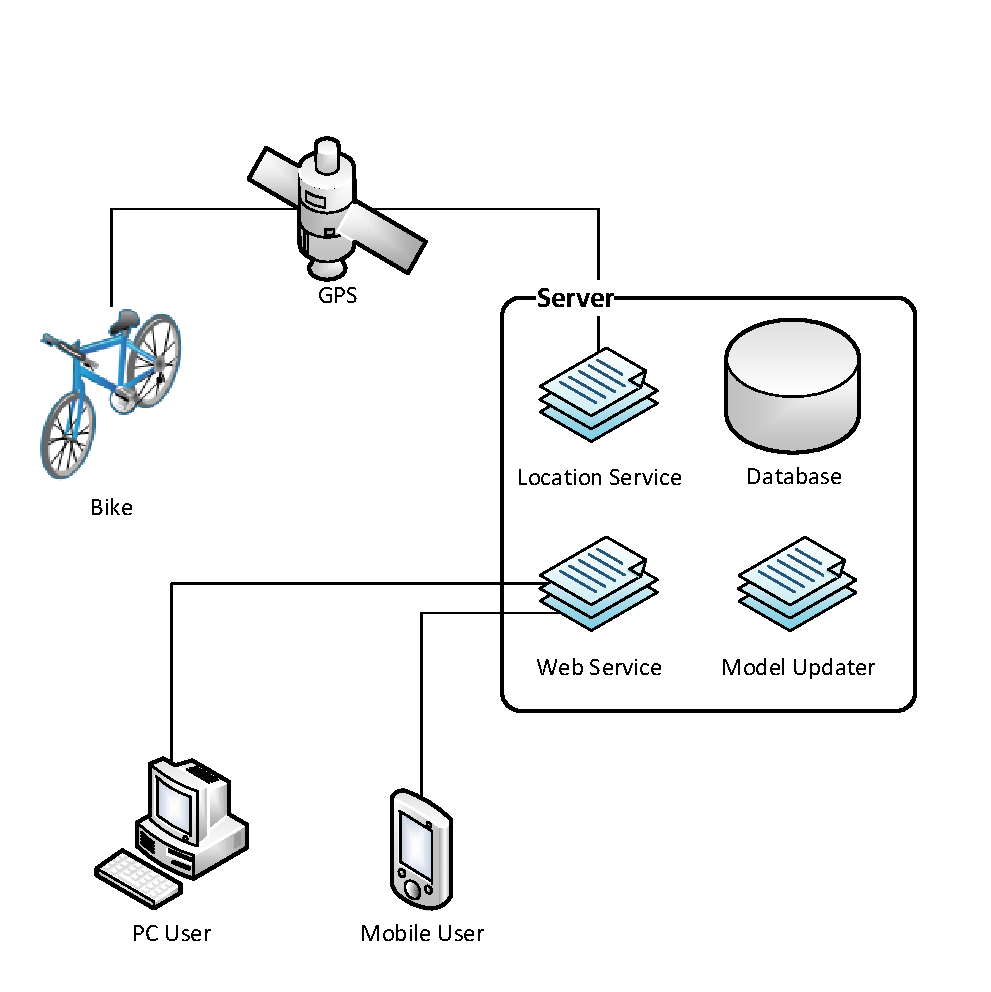
\includegraphics[width=\textwidth]{our_solution.pdf}
\caption{The overall structure of our solution}
\label{fig:solution_structure}
\end{figure}

The \textit{Location Service} continuously updates the locations of the bikes.
The \textit{Model Updater} uses the location updates to generate a model used for predictions.
The \textit{Webservice} makes available an API, in order to make platform implementations to make available the data as specified in the requirements.
